\documentclass[a4paper,man,natbib]{apa6}
%\usepackage[square]{natbib}
\usepackage{microtype}
\usepackage{mathtools} % needed
\usepackage{hyperref}
\usepackage{tabularx}
\newcolumntype{Y}{>{\raggedright\arraybackslash}X}

\usepackage[normalem]{ulem}
\hypersetup{hidelinks=True}
\usepackage{lingex} % some linguistic-style example numbering

\newcommand*{\smex}[1]{\textit{#1}} % 'small example'
\newcommand*{\spex}[1]{``{#1}''} % 'spoken example'
\newcommand*{\term}[1]{\emph{#1}} % introducing a new term
\newcommand*{\citegen}[1]{\citeauthor{#1}'s~(\citeyear{#1})}
\newcommand*{\SE}{\mathit{SE}} % fix funny "SE" spacing
\newcommand{\resultsLog}[3]{$\beta = #1$, $\textnormal{SE} = #2$, $p #3$}
\newcommand{\resultsLM}[3]{$\beta = #1$, $\textnormal{SE} = #2$, $t #3$}

\title{<Martin's pithy title about gesture and speech>.}
\author{JK, MC, HR}
\affiliation{Psychology, PPLS, University of Edinburgh}
\ifapamodeman{\note{\begin{flushleft}%
Josiah King\\
Philosophy, Psychology and Language Sciences\\
University of Edinburgh\\
7~George Square\\
Edinburgh EH8~9JZ, UK\\[1ex]
\url{J.P.J.King@sms.ed.ac.uk}
\end{flushleft}}}

\shorttitle{e5 - gesture production}

\abstract{                   
When a task becomes more conceptually demanding, speakers tend to produce more gestures.  
Previous research pins this increase either on gestures helping the speaker to package more complex information into appropriate units for speech, or on some of the communicative load being traded off from speech to gesture.  
The former view holds that speech and gesture co-vary, increasing in parallel with cognitive load.
The latter account suggests the inverse: A negative relationship between speech and gesture indicating a transference of communicative load to whichever modality is least difficult. 


%JK Hannah doesn't like "naturalistically occurring" and I'm inclined to agree. Don't have a suitable alternative though.
In the present study we elicit semi-naturalistic dialogues, and measure the relative durations of gestures and speech directly, in order to establish whether they co-vary (as would be predicted by the packaging account) or correlate inversely (as would be predicted by a trade-off).
Pairs of participants took part in a shape-matching game, alternating in the roles of director and matcher. 
Directors saw two shapes (one easy, one difficult) for two seconds, and subsequently described them to their partner.

In line with an information packaging account, speech duration and gesture duration increased in parallel for easy-to-name objects.
Importantly, when participants were referring to objects which were more difficult to verbally encode, gesture duration increased at a higher rate than speech duration.
This suggests that, when naming difficult objects, gesture does more than simply help the speaker to package verbal information.  Instead, gesture serves an additional communicative purpose, adding to, but not trading off against, the verbal descriptions which are uttered.
}

\begin{document}
\maketitle

\noindent
During conversation, speakers often move their hands and arms in meaningful ways which co-express the content of their speech \citep{McNeill1992}: %JK is this a bad opener, given that we're asking how much of gesture "co-expresses" speech and how much it takes over?
These movements might add emphasis to speech, indicate location, or depict properties of objects, movements, actions or space.
Research suggests that when a task becomes more conceptually demanding, speakers tend to produce more gestures.
This might be because gestures have benefits for speech, either in aiding lexical access \citep{Rauscher1996, Krauss2000} or in helping to wrap information into speech \citep{Kita2000}.
Alternatively, gesture production might increase with conceptual demand because some of the communicative load is being traded off from speech to gesture \citep{Melinger2004, Bangerter2004, DeRuiter2006}.

In contrast to common methods of measuring the number of discrete gestures per word, experimental trial or some other construct, the present study measures the relative durations of gestures and speech directly, in order to establish whether they co-vary (as would be predicted by a gesturing-to-benefit-speech account) or correlate inversely (as would be predicted by a trade-off).
With few studies having investigated the speech-gesture relationship in a dialogical setting where two people are making explicit contributions, we elicit semi-naturalistic dialogues in which participants jointly engage in producing referring expressions.

Although gesturing has traditionally been treated as a direct intent to communicate meaning to an addressee, recent research has suggested that it may in part be motivated by the cognitive benefits it has for the speaker.
Advantages of gesturing have been found in many areas: In speech production and planning processes \citep{Rauscher1996, Krauss1999, Rose2001, Morsella2004, Kita2000}; spatial working memory \citep{Wesp2001, Morsella2004}; conceptual planning \citep{Melinger2007}; and even doing mental arithmetic \citep{Goldin-Meadow2001}.

Explanations of the mechanism by which gesturing may benefit production of speech have been varied. 
One suggestion holds that gesturing increases activation on relevant items in the mental lexicon, thus facilitating access \citep{Krauss2000}. 
Another \citep{Hadar1997} suggests that gesturing prevents visuo-spatial imagery from decaying, providing speech production processes with higher quality information. 
In a similar vein, the Information Packaging Hypothesis \citep{Kita2000, Kita2003} claims that gesturing helps speakers to package complex information into appropriate units for speech. 

Common to all these accounts is the claim that as conceptual load increases, speech and gesture increase in parallel.
A \citeyear{So2009} study from \citeauthor{So2009} found evidence which patterned with this claim. 
Participants were asked to describe scenes from videotaped vignettes (e.g., a man giving a woman a basket), and their use of both speech and gesture to indicate characters in the scene was measured.
\citeauthor{So2009} found that speakers more often used a gesture to identify a referent if it was also specified in speech. 
\citeauthor{So2009} viewed their results as evidence in support of an account of speech and gesture going `hand-in-hand' --- i.e. the two modalities co-varying.

In contrast to \citeauthor{So2009}'s evidence for co-variance, other studies point to the use of gesture to compensate for underspecifications in their spoken descriptions.
For an example, in a communication task about spatial arrangements of connected dots of different colours where it was possible to determine the minimal content necessary for each stimulus, \citeauthor{Melinger2004} (\citeyear{Melinger2004}) examined whether omissions in speech were accompanied by compensatory gestures. 
\citeauthor{Melinger2004} found that people who gestured produced more --- and different --- omissions in speech than people who did not. 

\citeauthor{Melinger2004}'s findings pattern with other studies \citep{Bangerter2004, DeRuiter2006, VanderSluis2007} in which the informational content of speech is found to inversely correlate with the amount or precision of gestures. 
These findings point to a trade-off account which holds that speakers distribute communicative load across speech and gesture such that that when speaking becomes more difficult, gesturing will increase (and vice versa). 
This view directly contrasts with the co-varying account, suggesting that as it becomes harder to verbally encode meaning, rates of speech will decrease while rates of gesture will increase. 


%%%%%%%%%%%JK fix the two following paragraphs
To directly test the trade-off account, several studies have measured gesture production while manipulating the effort required to formulate spoken descriptions. 
\citet{DeRuiter1998} found that gesture rate did not change depending on whether speakers were describing simple arrangements of shapes and vertical/horizontal lines or random arrangements of shapes and diagonal lines.
However, as \citet{Morsella2004} point out, what \citeauthor{DeRuiter1998} varied in his stimuli was complexity, and not describability. 
In an experiment designed to tease apart these two concepts, \citet{Morsella2004} concluded that while visual complexity did not affect gesture rates, verbal codability did, with harder-to-name pictures (squiggles) eliciting higher rates of gesturing than easy-to-name pictures (familiar objects).

One explanation of the contrasting accounts of the speech-gesture relationship is that some types of gesture may be intended to communicate in place of speech (i.e. "A building with a roof like this [gestures a pointy roof]") while others might not.
There is some evidence for the communicative intent of gestures: \citet{Alibali2001} found that speakers who could see their addressee used more \term{representational} gestures, but not \term{beat} gestures. 
Similarly, \citet{DeRuiter2012} found mutual visibility to increase both pointing and \term{obligatory iconic} gestures (gestures containing information not represented in speech but required for disambiguation), but not \term{non-obligatory iconic} gestures (gestures which are not essential to the understanding of co-occurring speech).
However, \citeauthor{DeRuiter2012}'s \citeyear{DeRuiter2012} study found no evidence of a speech-gesture trade-off for \emph{any} type of gesturing, with speakers' gesture rates not changing depending upon whether referring to simple, humanoid or abstract tangrams. 


A further explanation for the differing findings is the variability in how speech and gesture have been measured. 
Previous studies have varied widely in their choice of measures for both modalities.
Tending towards \term{rate} measures (i.e. gesture as a function of speech), the predominant strategy has involved measuring the number of discrete gestures produced when speaking (e.g. \citet{Hostetter2007, Gerwing2011, DeRuiter2012, Hoetjes2015}).
Unlike speech --- where distinct phonemes and words offer comparatively clear means of measuring utterance length and duration --- multiple pieces of information (and multiple types of gesture) may be produced in the time between the raising and lowering of hands.
In the literature, defining individual gestures has varied with the thing being described, from ``illustrating a feature of the target (for instance its shape)'' when describing tangram figures \citep{DeRuiter2012} to change in any one of ``shape and placement of the hand, trajectory of the motion'' when identifying referents in a narrative \citep{So2009}.
On the side of speech, these measures of discrete gestures have then been calculated per trial \citep{Morsella2004}, per minute \citep{Mol2011}, per 100 words \citep{Masson-Carro2015, Hostetter2007, Gerwing2011, Hoetjes2015}, per \term{feature description} \citep{DeRuiter2012} or per \term{semantic attribute} \citep{Hoetjes2015}.

Because gestures and vocalisations can vary in durations, these metrics fail to capture the relative contributions of each.
We propose a duration-based approach in which relative durations of speech and gesture are measured directly.
By comparing the durations for which a speaker conveys (or attempts to convey) information via different channels when referring to either easy-to-name or hard-to-name shapes, we aim to establish whether speech and gesture trade-off against one another or co-vary.
On a broad level, the two accounts would simply predict a correlation between durations of speech and gesture but in different directions: A positive correlation suggests speech and gesture increase hand-in-hand, an inverse correlation suggests a trade-off.
Furthermore, a trade-off account would predict a stronger inverse correlation for easy-to-name shapes, whereas a hand-in-hand account would predict no difference for our manipulation of referent-nameability.
%JK would it predict a stronger correlation? or would it just predict a different intercept?

%JK this bit doesn't really fit.....
In addition to this new metric, our study targets investigating the speech-gesture relationship in a more ecological setting. 
To date, much of the research into gestures has involved studies in which a single speakers' gestures are evaluated under various conditions.
Experimental paradigms have tended towards those in which participants produce speech and gesture either to an imagined future addressee (e.g. \citet{Morsella2004, Wesp2001}) or to an addressee who is present but in a comparatively passive role (e.g. \citet{DeRuiter2012, Bangerter2004, Holler2007, Hoetjes2015}).
However, both of these designs fail to capture the dynamic process of conversation. 
Dialogue is often considered to be a joint activity \citep{Clark1996}, and gesture is no exception to this.
In \citet{Bavelas2008}, results suggested independent effects of visibility and dialogue on gesturing: Speakers produced more gestures when speaking to an occluded but dialogically involved listener than when speaking to a tape recorder. 
With this in mind, the present study elicits semi-naturalistic dialogues in which both participants make contributions. 


\section{Experiment}

Pairs of participants engaged in a collaborative matching game, in which they were tasked with matching two target shapes seen by one particpant from a set of six shapes seen by the other participant. 
Participants took turns in the roles of \term{director} and \term{matcher}.
Target shapes varied in verbal codability --- they were either easy- or hard-to-name.
We also manipulated participants' familiarity with the target shapes in both roles (director and matcher) --- descriptions referred to either a previously named target, a previously viewed target, or a novel one.


\subsection{Materials}
Pairs of shapes in critical trials were selected from a set of 20 critical shapes (10 easy-to-name, 10 hard-to-name).
Each of the 10 easy-to-name shapes was altered (sections of the shape were rotated and/or flipped) to create the 10 hard-to-name variants. %JK see fig!
For filler trials, shapes were selected from a further set of 40 shapes (20 easy-to-name shapes and 20 hard-to-name variants). 

A set of 20 \term{distractor} shapes (10 easy-, 10 hard-to-name) were visually and descriptively similar to the 20 critical target shapes. %JK REWORD, give example
These shapes were never described, only being presented as part of the matchers' arrays, with the aim of encouraging specificity in descriptions.

The director's array was always comprised of only two shapes.
In critical trials these shapes differed in codability (one easy-to-name and one hard-to-name), and in filler trials they were both of the same codability (both easy-to-name or both hard-to-name).

The matchers' array was comprised of six shapes.
Along with the two target shapes for that trial, this set contained two randomly selected filler shapes and two randomly selected distractor shapes. 
Codability of the shapes in the array matched that of the target shapes (i.e. for critical trials, half were easy-to-name, half were hard-to-name).
Shapes were randomly positioned for both the director (Left vs.\@ Right) and for the matcher (in a 2x3 grid).


\subsection{Experimental blocks}

The experiment consisted of two blocks, each containing 40 trials (20 critical and 20 fillers). 
In each block, every critical shape was seen twice.

In the first block, trials were sampled randomly from a set of 20 critical trials (in which each critical shape was present in two trials) and 20 filler trials (in which two shapes of the same codability were randomly selected from the set of filler shapes). 
Selection was constrained such that shapes were never repeated in consecutive critical trials.
Whilst the majority of the shapes were described once by each participant, the probability that a given shape was described twice by the same participant was 25\%.\footnote{Whilst the intention was to make it so that each participant described each critical shape once, a typing error in the experiment script resulted in these distributions} 

In the second block the goal was to get a measure of behaviour for familiar objects 
In the second block, pairs of consecutive critical trials alternated with pairs of filler trials. 
For the consecutive critical trials, the difficult-to-name shape was repeated.
This meant that for critical trials where participant B was the director, they were tasked with describing the difficult shape which had just been described to them in the previous trial by participant A.

Filler trials, like for block 1, consisted of two randomly selected shapes of the same codability from the set of 40 filler shapes. 


\subsection{Procedure}
Participants sat facing one another with an unobstructed space between them.
Each participant had a monitor and a mouse on a table to their left, positioned such that they could not see what was on their partner's monitor.
The setup was designed to encourage face-to-face dialogue, and to discourage participants from leaving their hand resting on the mouse whilst speaking (the position being uncomfortable for a right-handed mouse user), thus leaving both arms free to gesture.
Audio and video was recorded by two cameras positioned to the right of each participant, facing their partner.

Taking turns in the roles of director and matcher, participants were tasked with successfully matching what was seen on the director's monitor from a set of possibilities on the matcher's monitor.

As a pair, participants were awarded points for successful matching.
As an incentive, the highest scoring pair received \pounds 40, and participants were informed of this beforehand.

A high-score table was shown prior to the experiment, with participants adding their score to the table after they had played.
Participants were asked to restrict their communication to within the 10 second time-window during which no images were present on either screen. 
The onset of this period was signalled by the images disappearing from the director's screen, and the offset was marked by the sound of a bell (see Figure \ref{fig:trial}).
The aim of this was to encourage participants to look at their partners during communication, and not at their screens. 
Gesturing was permitted but not explicitly encouraged, as participants were told that during this period, they were "both allowed to talk, gesture, ask questions, and so on".

Feedback was given at the end of each trial (The number of correctly matched shapes was signified by an equivalent number of bell rings, with zero correct resulting in a buzzer), and the participants' cumulative score was displayed.

\begin{figure}
  \centering
	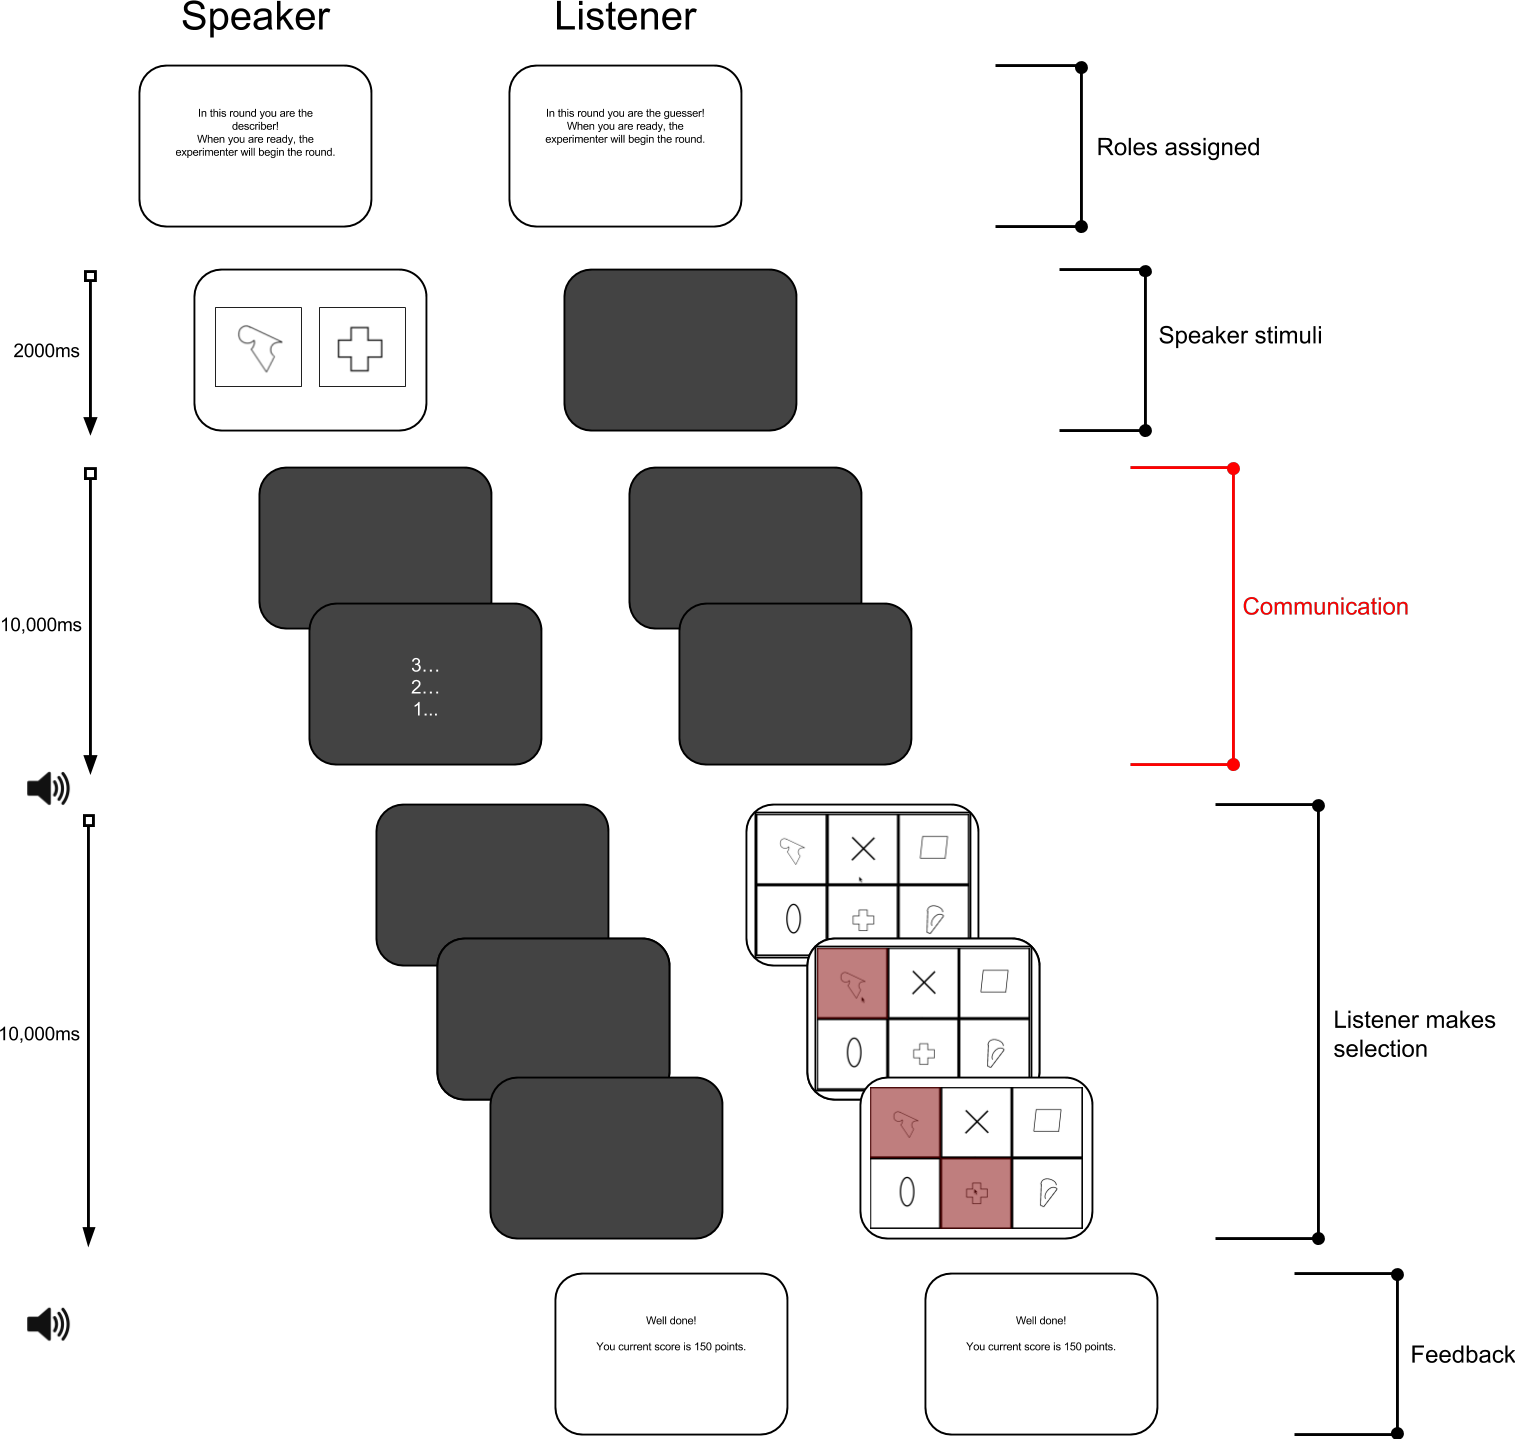
\includegraphics[width=\linewidth]{trial.png}
  \caption{Procedure of a given trial.}
  \label{fig:trial}
\end{figure}

\section{Coding}
Audiovisual data for each pair of participants was coded using a three stage process:
Audio-only and Video-only stages were used to code for speech and gesture respectively, with the third stage (both Audio and Video) used to confirm the annotations resulting from the previous stages.
As each trial consisted of describing two shapes, special care was taken in the third stage to ensure that utterances and gestures were assigned to the correct referents.\footnote{There was potential for descriptions in both modalities to be interleaved}



\subsection{Speech Coding}
Utterance duration, utterance length and disfluencies were coded in the Audio-only stage.
Within each trial, only the first mention of each shape was used. 
Utterance duration (ms) was coded from the onset of the noun-phrase up until either a) speech-offset, or b) a valid interruption from the listener in either modality.
Listeners' use of the collateral channel (for instance: "yep","mmhm",[nods head]) were not considered valid interruptions.
Utterance length (number of words) was coded analogously, with disfluencies within the utterance period being identified and excluded from this measure.

Disfluencies were coded as falling into one of six categories: Filled pauses; Insertions; Substitutions; Articulation Errors; Deletions; Repetitions (see \citet{Shriberg1996}).
Any speech prior to the onset of the noun-phrase was coded as either fluent or disfluent.

%JK Conceptual pacts were coded during the third (both Audio and Video) stage. 
%JK HOW DO WE CLASSIFY CONCEPTUAL PACTS. definite descriptions "THE","again","another". 



\subsection{Gesture Coding}
Gestures were identified in the Video-only stage of the coding process.
Any movement from the fingers up to the shoulder were considered. 
Only gestures which partially overlapped an identified utterance period were included, and were assigned to the utterance which they primarily overlapped. 
This pairing was then confirmed in the third stage of the coding process. 
In any cases of a gesture being ambiguous as to which utterance it accompanied (i.e. non-representational gestures which overlap both utterance periods), the gesture was assigned to both referents.

Gestures were categorised into five types: Iconics; Beats; Points; Adaptors; and Others. 
Any gesture which was considered to be an attempt to represent any feature of the target shape was coded as an Iconic gesture.
Beat gestures were identified as any movements which rhythmically matched prosody in speech but which \emph{did not} represent any feature of the target shape.
Point gestures were extensions of the index finger used to refer deictically to either present objects or people, or to previous parts of the discourse.
%JK give examples ?
Other movements were categorised as either adaptor gestures (scratching, stroking, manipulating clothing, etc.), or other miscellaneous gesticulations.

Individual gestures were identified by onset of movement, and continued either until the start of the retraction phase, or until transformation into a) a different category of gesture or b) iconic gesturing referring to a different shape (i.e. the other shape in the trial).

The third stage of the coding process (audio and video) was used to confirm the coding of the first and second stages, specifically gesture categorisation and pairing of gestures with referents.
Several gestures remained ambiguous between iconic and beat even after this third stage (n referencing easy shapes, and n referencing difficult shapes).%JK N=? fill in 
These were considered to be imprecise/lax attempts at representing the shapes in space, and thus coded as iconic gestures.
Additionally, this stage was used to code whether or not the utterance referred explicitly to the gesture being made (e.g. "like this","like that","a bit here", etc.)

Once identified, iconic gestures were coded for gesture duration analogously to the measure of utterance duration:
Gesture duration for iconic gestures was measured from the onset of the first stroke or hold phase up until the retraction phase, or until interruption.
End-of-gesture hangs (uninformative hangs immediately prior to a retraction phase) were not included.\footnote{We discerned here between end-of-gesture \term{hangs} and end-of-gesture \term{holds} which continued to convey some representational content, and were thus included as part of gesture duration}

This measure of gesture duration included any hangs, false starts, or preparation which occurred within-gesture, just as utterance duration included within-utterance pauses and disfluencies.
Any suspected false starts and repetitions were counted (a finger trace which is subsequently reversed counts as repetition, as does a static hold with a distinct beat gesture incorporated).

Additionally, all gestures were coded for the hands used (Left, Right, or Both), and whether the representational part of the gesture was conveyed dynamically, statically, or as a combination of both. 

\subsection{Second rater}
For 20\% of critical trials, interrater agreement was measured for utterance duration, gesture duration and gesture type, with the second rater blind to the study aims (e.g. blind to the focus on the speech duration:gesture duration ratio).
%JK results of second coding.

%Additionally, we measured the change in positions of skin tone pixels (excluding the area surrounding faces) between video frames. 
%The durations of movements which overlapped utterance durations were included as an alternative measure of gesture duration.
%Whilst this metric cannot be used to separate preparatory and retraction phases from gestures, it provides an objective measure of how much participants moved whilst speaking about different referents.
%Unfortunately, this method is not yet sophisticated enough to identify gestural holds, and as such only captures the dynamic components of gesturing.

\section{Results}
\subsection{Analysis}
Analysis was carried out in R version~3.4.2 \citep{rbase}, using the lme4 package \citep{lme4}.
Only the critical trials were included in the analysis (1760 of the 3520 referring expressions elicited).
For trials in which participants made no attempt to describe one or both of the shapes --- either due to running out of time, forgetting to describe a shape, or appearing to forget what shape they had seen --- those descriptions were excluded from all analysis (0.7\% of referring expressions).

\paragraph{G vs No G}
On the remaining 1748 descriptions, the production (categorical gesture vs.\@ no gesture) of each type of gesturing (Iconic, Beat, Point, Adaptors, and Others) was modelled using mixed effects logistic regression. 
Verbal codability (easy-to-name vs.\@ hard-to-name), description number for each speaker (1-80) and their interaction were included as fixed effects, with random intercepts both by-participants and by-shapes and a by-participant random effect of verbal codability.
For all referring expressions accompanied by iconic gesturing (n = 1301), spoken reference to the gestural component of a description (``like this'';``a bit here'') was modelled with the same fixed and random effect structure.

\paragraph{relationship}
To investigate whether gesturing co-varies or trades off against speech, the duration of iconic gesturing (Z-scored) was analysed using mixed effects linear regression.
Utterance duration (Z-scored), Verbal codability, description number, and all interactions were included as fixed effects. 
Random intercepts and random slopes for utterance duration, verbal codability and their interaction were included by-subject, along with random intercepts and effects of verbal codability by-shape.

\paragraph{gestures and disfluencies}

\paragraph{gesturing and familiarity with shapes}
Given the experimental design, it was possible to code each speakers familiarity with 
















\begin{figure}
  \centering
	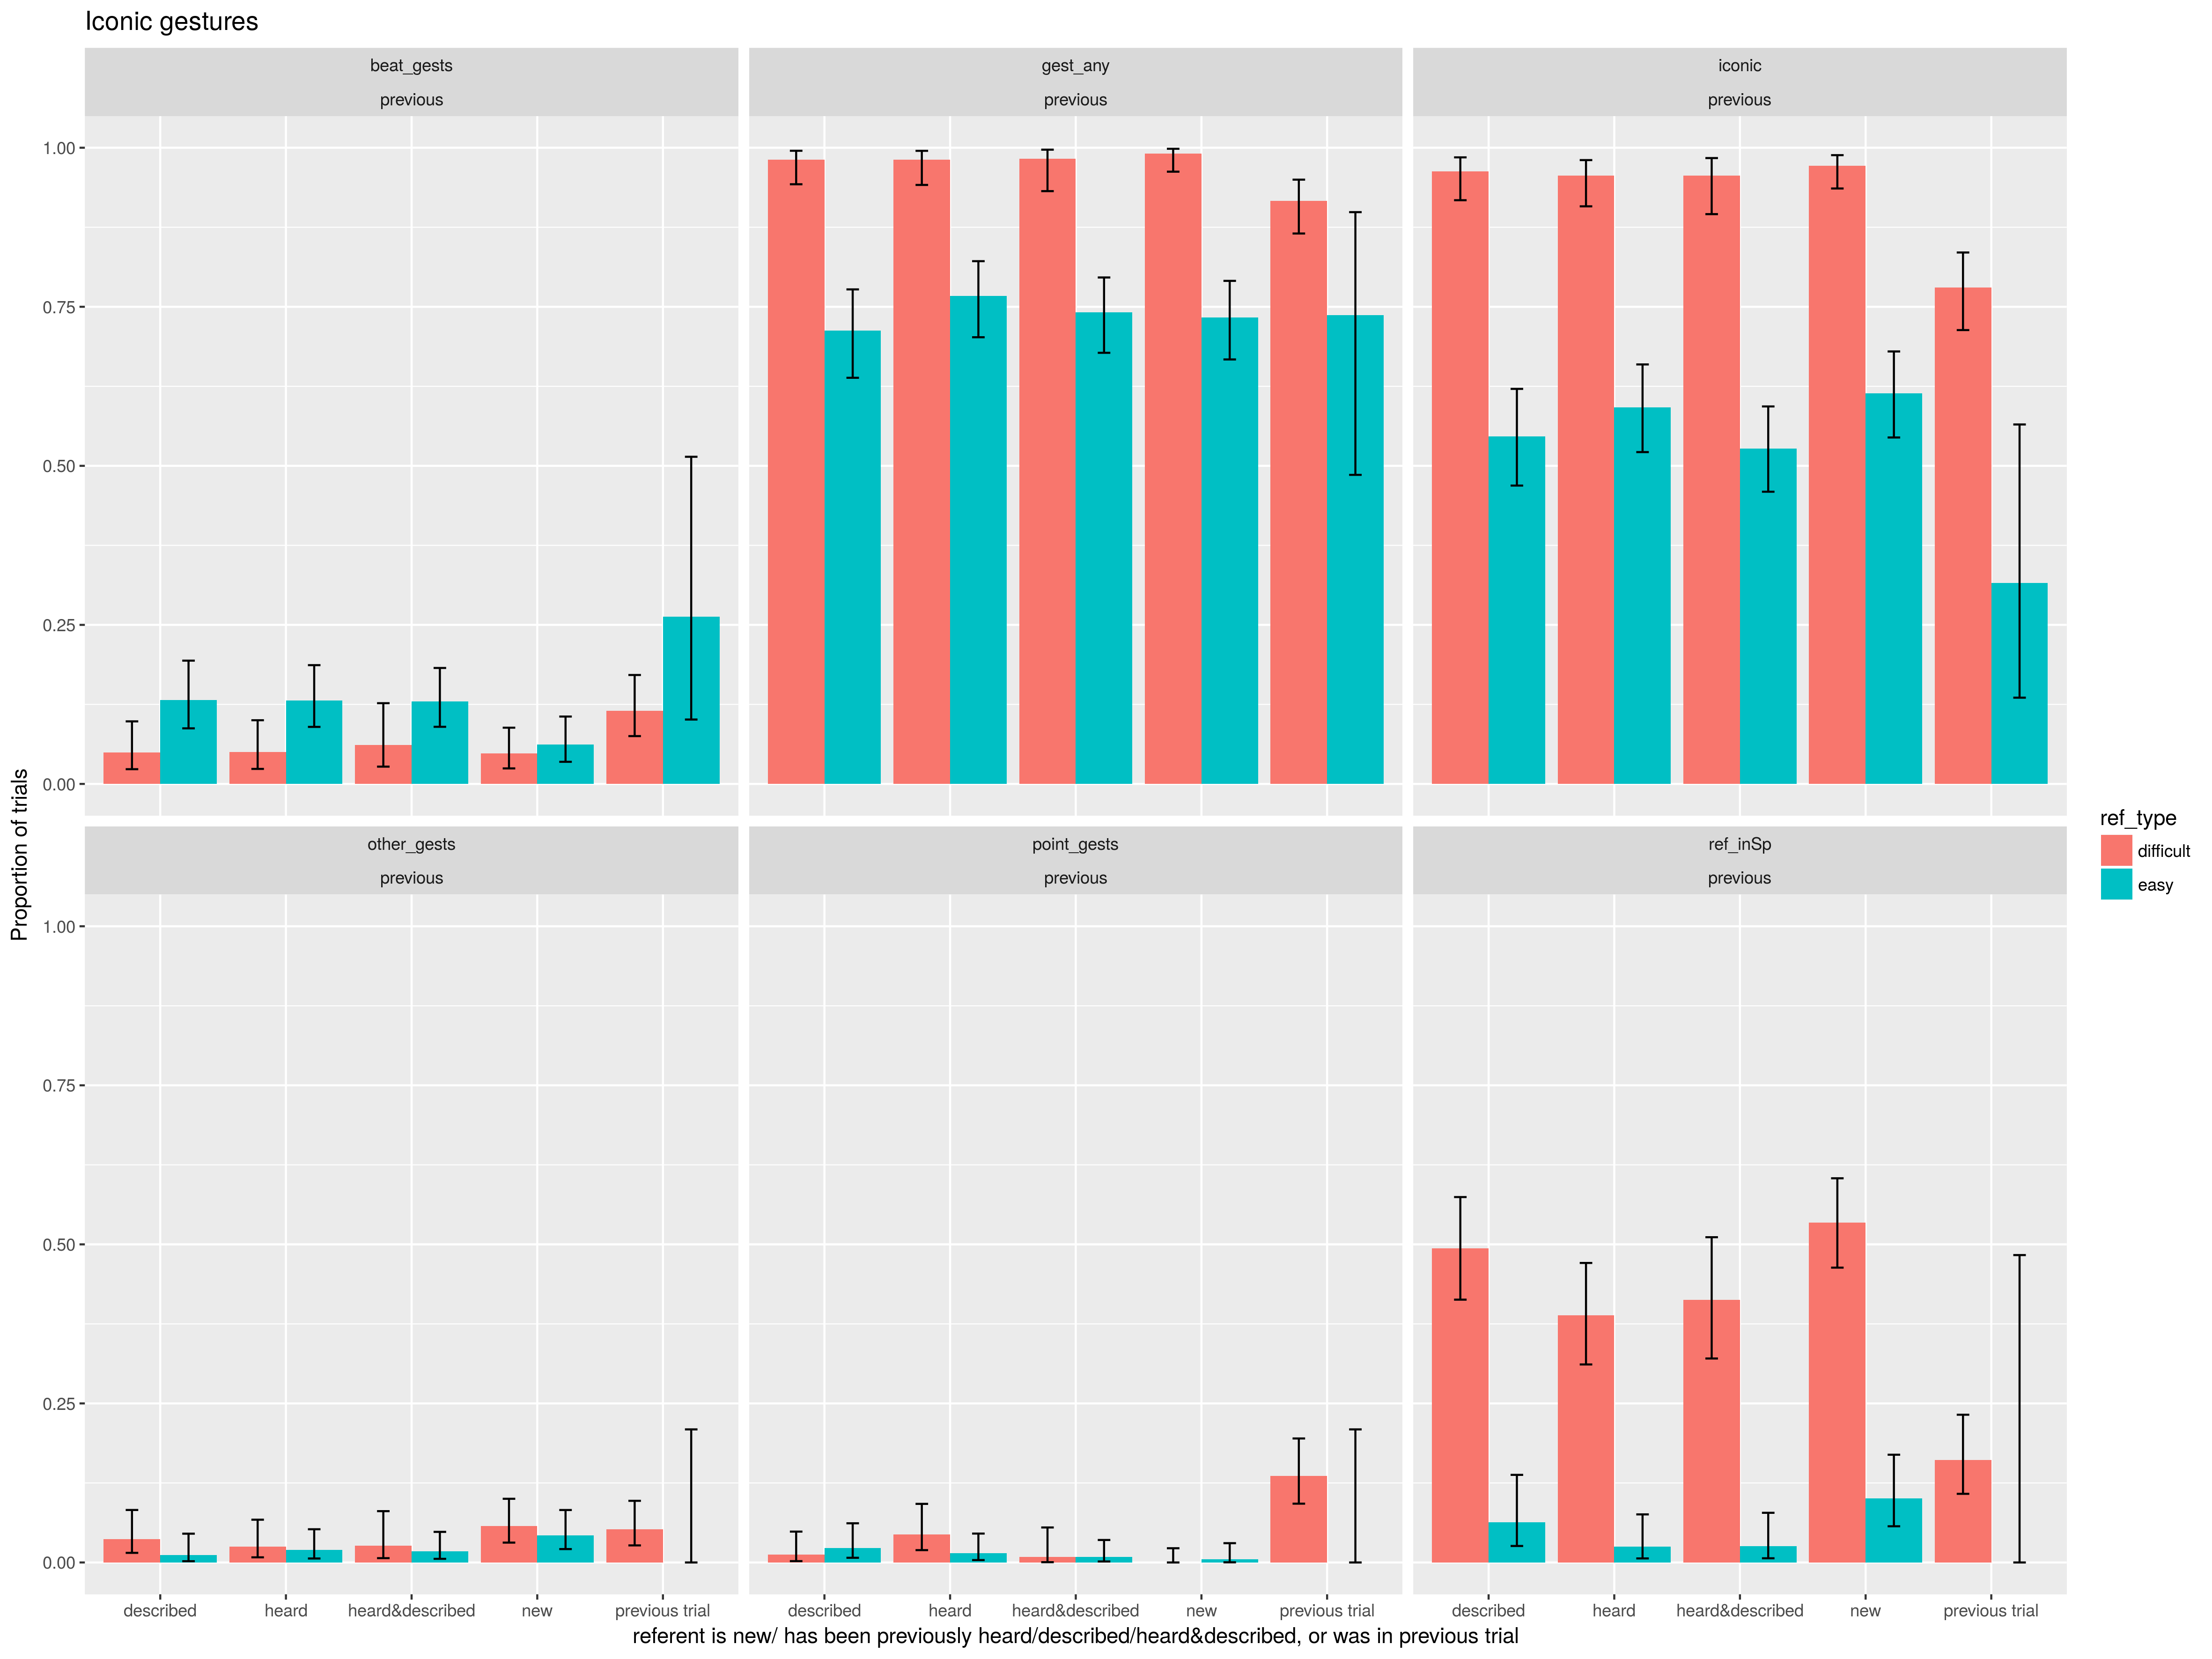
\includegraphics[width=\linewidth]{previousplot.png}
  \caption{gestures}
  \label{fig:plot}
\end{figure}

\section{discussion}
duration measures - pros and cons.
where to measure from. hangs etc. 
when is iconic iconic? when is it beat? - also applies to other measures 
describability vs complexity

driven by two things.
descriptions of easy shapes which are familiar, but have a longer utterance ("a circle, just the normal circle we've seen lots")
and descriptions of difficult shapes with oblig iconics ("like this"[long gesture]")



\bibliography{e5}

\end{document}
%%% Local Variables:
%%% mode: latex
%%% TeX-master: t
%%% End:
